\documentclass{article}
\usepackage{v-equation}
\vgeometry

\begin{document}

\def\gdrive{https://drive.google.com/drive/folders/141zKhEJynQDMqgtmW9NSM4S-NshCWVMy?usp=share_link}

\vtitle[Time Period of the charge in the magnetic field]

\begin{center}
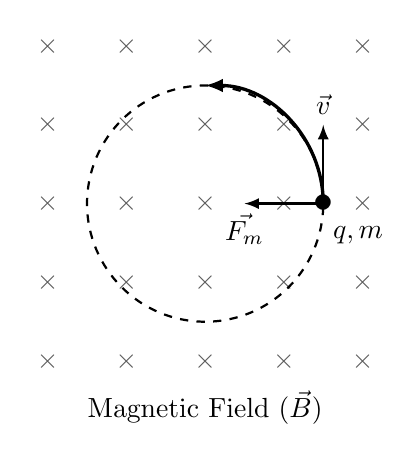
\begin{tikzpicture}
[xscale=1, yscale=1, >=latex]
\foreach \x in {-2,...,2} \foreach \y in {-2,...,2} { \node at (\x, \y)[opacity=0.65]{$\times$};}
\draw[thick,dashed] (0,0) circle[radius=1.5];
\node at (1.5,0)[below=4 mm, right]{$q, m$};
\draw[->, thick] (1.5,0)--(1.5,1)node[above]{$\vec{v}$};
\draw[->, thick] (1.5,0)--(0.5,0)node[below]{$\vec{F_m}$};
\draw[->, very thick] (1.5,0) arc[start angle=0, end angle=90, radius=1.5];
\node at (0,-2.25)[below]{Magnetic Field ($\vec{B}$)};
\node at (1.5,0) {\Large{$\bullet$}};
\end{tikzpicture}
\end{center}
\vspace*{\fill}
\begin{align*}
T & = \dfrac{2\pi}{\omega}\\
  & = \dfrac{2\pi}{\left(\dfrac{v}{r}\right)} &&\omega = \dfrac{v}{r}\\
  & =\dfrac{2\pi r}{v} &&r=\dfrac{mv}{qB}\\
T & = \dfrac{2\pi m}{qB}
\end{align*}
\vspace*{\fill}

\pagebreak

\vspace*{\fill}
\begin{center}
    \fbox{\qrcode[height=2cm]{\gdrive}}
\end{center}
\vspace*{\fill}
\end{document}
